\documentclass[10pt,twocolumn]{article}
\usepackage[a4paper,margin=1.45cm,top=1.1cm,bottom=1.1cm]{geometry}
\usepackage[T1]{fontenc}
\usepackage{lmodern}
\usepackage{microtype}
\usepackage{amsmath}
\usepackage{booktabs}
\usepackage{graphicx}
\usepackage{caption}
\usepackage{titlesec}
\usepackage[hidelinks]{hyperref}
\captionsetup{font=small,labelfont=bf,skip=3pt}
\titlespacing*{\section}{0pt}{7pt}{3pt}
\titlespacing*{\subsection}{0pt}{5pt}{2pt}
\titleformat*{\section}{\normalsize\bfseries}
\titleformat*{\subsection}{\small\bfseries}
\setlength{\columnsep}{0.65cm}
\setlength{\parskip}{0pt}
\setlength{\abovecaptionskip}{3pt}
\renewcommand{\arraystretch}{1.08}
\graphicspath{{figures/}}

\title{\vspace{-1.1cm}\large\bfseries Store placement by quantum minimum finding:\\D\"urr--H{\o}yer search on real census and road data at 10--12 qubits}
\author{\normalsize Team ZollerQu (Tushar Pandey, Oussema-t)\\\small Qollab $\times$ IonQ Hackathon, 9--11 October 2026 \quad---\quad This effort is supported by Qollab \& IonQ.}
\date{}

\begin{document}
\maketitle
\vspace{-0.9cm}

\begin{abstract}\noindent
We place $k=4$ stores among $m$ candidate sites in Champaign County, Illinois, using 2020 census block-group populations and OpenStreetMap driving times. The cost combines travel, staffing, crowding and warehouse supply and is minimised exactly by scanning all $N=\binom{m}{k}$ feasible placements. The quantum method is D\"urr--H{\o}yer minimum finding: Grover search over the same $N$ placements, started in the Dicke state $|D(m,k)\rangle$, with a threshold oracle that tightens after each single-shot round. On an exact statevector simulator at $m=12$ ($N=495$) the measured Grover success probabilities lie within 2.8 percentage points of $\sin^2((2j+1)\theta)$ over 31 circuits, the loop returns the exact minimum after scoring 170 placements against 495 for the scan, and over 65 runs at $N=15$ to $495$ the mean number of placements scored is $7.3\sqrt N$ with the exact minimum reached every time. The oracle is a lookup table compiled from the classical cost table, so no speedup is claimed at this size; the claim is that the circuits behave as the theory predicts, and the $O(\sqrt N)$ bound is the theory's. Everything runs on the Qollab page; the IonQ Forte simulator run replaces the local take when available.
\end{abstract}

\section{Problem and data}
\textbf{Data.} 158 census block groups of Champaign County, IL (US Census Bureau TIGERweb, Census 2020 Block Groups, layer 11; total population 205\,865) with centroids; 12 candidate store sites at the centroids of the most populous block groups, thinned so that every pair is at least 4 driving minutes apart (the closest pair is 4.1); two warehouse candidates at the east and west edges of the county. Driving minutes between every block and site, site and site, and warehouse and site come from the OSRM demo server (OpenStreetMap roads). Everything is fetched without API keys by \texttt{tools/build\_data.py} and shipped as one JSON file.

\textbf{Cost.} A placement is a subset $S$ of the first $m$ sites with $|S|=k$; any other bit count is infeasible. With block population $p_b$, travel minutes $t_{bi}$ and $t_{ij}$, and warehouse-to-site minutes $t_{wi}$,
\begin{equation}
\begin{aligned}
C(S) ={}& \frac{\sum_b p_b \min_{i\in S} t_{bi}}{\sum_b p_b}
      + 3.0 \sum_{i\in S} \Big\lceil \tfrac{P_i(S)}{15\,000} \Big\rceil \\
     &+ 10 \,\big|\{\,\{i,j\}\subset S : t_{ij} < 10\,\}\big| \\
     &+ 0.1 \min_w \sum_{i\in S} t_{wi},
\end{aligned}
\end{equation}
where $P_i(S)$ is the population assigned to site $i$ (nearest open site). The four weights are sliders on the page; the defaults above were chosen by a scan so that the landscape is not trivial: at $m=12$ greedy misses the optimum by 1.8 cost units and steepest-descent local search from 20 random starts reaches 5 distinct local minima.

\section{Methods}
\begin{figure*}[t]\centering
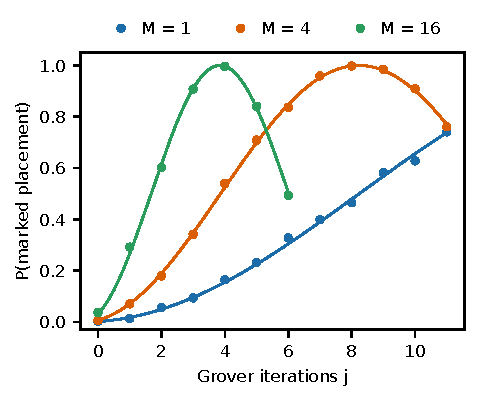
\includegraphics[width=0.32\textwidth]{sweep}\hfill
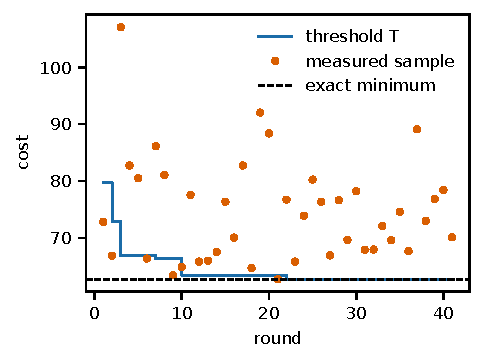
\includegraphics[width=0.32\textwidth]{rounds}\hfill
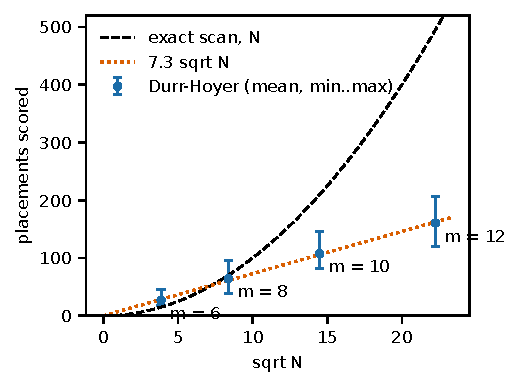
\includegraphics[width=0.32\textwidth]{scaling}
\caption{Left: theory-match sweep. Markers: measured probability of sampling a marked placement, 1\,000 shots per circuit; lines: $\sin^2((2j+1)\theta)$. Largest deviation 2.8 points ($M=1$), 1.5 ($M=4$), 2.6 ($M=16$). Middle: the shipped D\"urr--H{\o}yer loop (seed 7, one measurement per round). The threshold reaches the exact minimum in round 21 (41 placements scored); the remaining 20 rounds are the stop rule. Right: scaling study, one measurement per round, simulator seed $=\text{seed}\times1000+\text{round}$; mean placements scored with min--max bars over 20 seeds ($m=6,8,10$) and 5 seeds ($m=12$); dashed: the exact scan's $N$; dotted: least-squares $7.3\sqrt N$.}
\label{fig:row}
\end{figure*}

\textbf{Classical baselines} (NumPy, from the same cost table): exact scan of all $N=\binom{m}{4}$ feasible placements ($N$ placements scored); greedy, adding the site with the best marginal cost $k$ times (it scores partial placements, which are not table entries, so its count is reported but not compared); local search, swapping one open site for one closed site, steepest descent from 20 random feasible starts.

\textbf{Quantum minimum finding.} D\"urr and H{\o}yer~\cite{dh} find the minimum of an $N$-entry table with $O(\sqrt N)$ oracle calls: keep a threshold $T$, run Grover search for an entry with cost $<T$, measure once, and lower $T$ to the measured cost if it improved. We start the register in the uniform superposition over feasible placements only, the Dicke state $|D(m,k)\rangle$, prepared by the deterministic circuit of B\"artschi and Eidenbenz~\cite{dicke} ($O(km)$ gates, no ancilla; 246 CNOTs at $m=10$), and the diffusion operator reflects about that state, so the quantum search space is the same $N=\binom{m}{k}$ as the classical scan. Because the number of marked entries is unknown, the Grover iteration count $j$ in each round follows the Boyer--Brassard--H{\o}yer--Tapp exponential schedule~\cite{bbht} (budget grows by $6/5$ per idle round up to $\sqrt N$). One counting rule on both sides: placements scored. The loop scores one placement for its random start, one per Grover iteration (one oracle call each) and one per round for the measured sample. The loop stops after three idle rounds at the largest budget (a project heuristic, not the paper's time bound) or after 120 rounds.

\textbf{The oracle, stated plainly.} The threshold oracle is a diagonal gate with phase $-1$ on every placement with cost below $T$, compiled from the classical cost table. It is a lookup table, not an arithmetic circuit: a reversible circuit computing $C(S)$ from 158 block populations does not fit in the 29 qubits of the largest Qollab simulator. All counters count oracle calls, which is the quantity the quadratic speedup is about; no wall-clock figure is reported. One Grover iteration (oracle, Dicke preparation twice, reflection) transpiles to 1\,846 CNOTs at $m=10$ and 5\,286 at $m=12$ in the $\{R_z, \sqrt X, X, \mathrm{CX}\}$ basis.

\textbf{Theory-match sweep.} Before the loop, three fixed thresholds marking $M=1$, 4 and 16 placements are run for $j=0,\dots,J$ Grover iterations with $J=\min(11,\lceil 1.2\cdot\tfrac{\pi}{4}\sqrt{N/M}\,\rceil)$, 1\,000 shots each (31 circuits at $m=12$), as one batched job. The measured fraction of shots on marked placements is compared with $\sin^2((2j+1)\theta)$, $\sin\theta=\sqrt{M/N}$. IonQ backends accept one job per run, so the sweep runs live there and the loop (one short job per round) runs live only on local simulators and is otherwise shown from the recorded take.

\textbf{Tests.} 54 unit tests cover the cost terms, feasibility mask, Dicke preparation, oracle marking, the counting rule, the sweep analysis and the bridge the page calls; the take is regenerated by \texttt{tools/record\_take.py} on Qiskit Aer.

\section{Results ($m=12$, $k=4$, $N=495$, Aer statevector)}
\begin{figure}[t]\centering
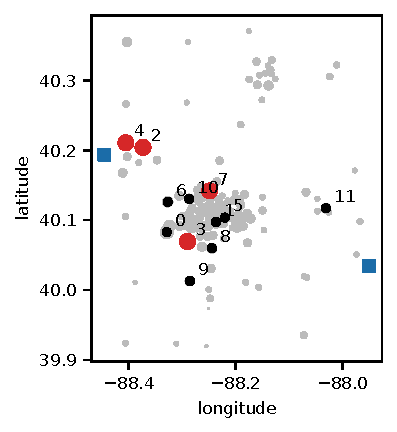
\includegraphics[width=0.58\columnwidth]{map}
\caption{Block-group centroids (grey, area $\propto$ population), the 12 candidate sites (numbered), the optimal four (red) and the two warehouse candidates (blue squares).}
\label{fig:map}
\end{figure}


\begin{table}[t]\centering\footnotesize\setlength{\tabcolsep}{4pt}
\caption{Shipped instance, default weights. Placements scored under one counting rule; greedy scores partial placements and is not compared; local search is 20 random starts and reached 5 distinct local minima.}
\begin{tabular}{@{}lccl@{}}\toprule
Method & cost & placements scored & sites\\\midrule
Exact scan & \textbf{62.73} & 495 & 2, 3, 4, 7\\
Greedy & 64.51 & (42 partial) & 1, 2, 4, 9\\
Local search & 62.73 & 1\,876 & 2, 3, 4, 7\\
D\"urr--H{\o}yer, seed 7 & \textbf{62.73} & 170 & 2, 3, 4, 7\\
\bottomrule\end{tabular}
\label{tab:main}
\end{table}

\textbf{Circuits match the theory.} Figure~\ref{fig:row} (left): over 31 circuits the largest gap between the measured success probability and $\sin^2((2j+1)\theta)$ is 2.8 percentage points, consistent with the binomial spread of 1\,000 shots. This is the check that the Dicke preparation, oracle and diffusion do what the algorithm assumes.

\textbf{The loop finds the exact minimum.} Table~\ref{tab:main} and Figure~\ref{fig:row} (middle): the seed-7 loop returns the exact optimum (cost 62.73, sites 2, 3, 4, 7, Figure~\ref{fig:map}) in 41 rounds with 128 Grover iterations, scoring $1+128+41=170$ placements against the 495 of the exact scan. The minimum is in hand after 41 placements; the rest is the stop rule. A single loop can stop short of the minimum (the paper guarantees success with probability at least $1/2$ within its budget); how often it does is the scaling study.


\begin{table}[t]\centering\footnotesize\setlength{\tabcolsep}{4pt}
\caption{Scaling study (same loop, random seeds).}
\begin{tabular}{@{}ccccccc@{}}\toprule
$m$ & $N$ & $\sqrt N$ & seeds & mean (min..max) & mean$/\sqrt N$ & exact\\\midrule
6 & 15 & 3.9 & 20 & 27 (18..46) & 6.9 & 20/20\\
8 & 70 & 8.4 & 20 & 64 (39..96) & 7.7 & 20/20\\
10 & 210 & 14.5 & 20 & 108 (82..146) & 7.4 & 20/20\\
12 & 495 & 22.2 & 5 & 161 (120..207) & 7.2 & 5/5\\
\bottomrule\end{tabular}
\label{tab:scaling}
\end{table}

\textbf{Calls grow like $\sqrt N$.} Table~\ref{tab:scaling} and Figure~\ref{fig:row} (right): as $N$ grows 33-fold the ratio of mean placements scored to $\sqrt N$ stays between 6.9 and 7.7, and all 65 loops reached the exact minimum. At $m=6$ the loop scores more placements than $N$: the constant in front of $\sqrt N$ wins at tiny $N$, as it must. The exact-minimum fraction is a property of this implementation's stop rule, not the paper's bound.

\section{What is proven, and what is not}
D\"urr and H{\o}yer~\cite{dh}: the minimum of an unsorted $N$-entry table is found with $O(\sqrt N)$ oracle calls with probability at least $1-1/2^c$ in time $O(c\sqrt N)$; any classical method needs $\Omega(N)$ calls in the worst case. Montanaro~\cite{montanaro}: branch-and-bound, the standard exact method for facility location and other mixed-integer programs, admits a near-quadratic quantum speedup in the size of the branch-and-bound tree. Not proven and not claimed here: any speedup on a 495-entry table on a simulator, or any wall-clock gain. The quadratic speedup needs a fault-tolerant machine and an arithmetic oracle; this entry shows the algorithm behaving as predicted, on real data, at the size that can be simulated, with the classical and quantum counts under one rule.

\textbf{Reproducibility.} Code, data, tests and the recorded take are in the \texttt{placement} branch of \url{https://github.com/Oussema-t/zollerqu-qollab} (MIT). On Qollab the page runs the sweep and the loop live on the built-in, Aer and Braket simulators; the figures in this report are produced by \texttt{paper/make\_figures.py} from the shipped take.

\begin{thebibliography}{9}\footnotesize\setlength{\itemsep}{0pt}
\bibitem{dh} C. D\"urr, P. H{\o}yer, A quantum algorithm for finding the minimum, arXiv:quant-ph/9607014 (1996).
\bibitem{dicke} A. B\"artschi, S. Eidenbenz, Deterministic preparation of Dicke states, FCT 2019, arXiv:1904.07358.
\bibitem{bbht} M. Boyer, G. Brassard, P. H{\o}yer, A. Tapp, Tight bounds on quantum searching, Fortschr. Phys. 46, 493 (1998), arXiv:quant-ph/9605034.
\bibitem{montanaro} A. Montanaro, Quantum speedup of branch-and-bound algorithms, Phys. Rev. Research 2, 013056 (2020).
\end{thebibliography}
\end{document}
